\documentclass{article}
% \usepackage[classica]{topfront}
\usepackage[utf8]{inputenc} %utf8
\usepackage[english]{babel}
\usepackage[T1]{fontenc}
% \usepackage{blindtext}
% \usepackage{wrapfig}
\usepackage{graphicx}
\usepackage{booktabs}
\usepackage{lmodern}
\usepackage{multicol}
\usepackage{physics}
\usepackage{varioref}
\usepackage{url}
\usepackage{array}
% \usepackage{paralist}{\obeyspaces\global\let =\space}
\usepackage{verbatim}
\usepackage{subfig}
\usepackage{tabularx}
\usepackage{amsmath}
\usepackage{accents}
\usepackage{slashed}
\usepackage{amsfonts}
\usepackage{float}
\usepackage{amssymb}
\usepackage{multicol}
\usepackage{multirow}
\usepackage{listings}
\usepackage[a4paper, total={5.5in, 8in}]{geometry}
\usepackage[figuresright]{rotating}
% \usepackage{algorithm}
% \usepackage{algpseudocode}
\usepackage{amsmath}
\usepackage{physics}
\usepackage{bbold}
\usepackage[babel]{csquotes}
\usepackage{hyperref}
\usepackage{mathtools}
\usepackage{subfig}
\usepackage{setspace}
\usepackage[sorting=none,style=numeric-comp,backend=biber]{biblatex}
\usepackage{tikz}
\usepackage{mathdots}
\usepackage{yhmath}
\usepackage{cancel}
\usepackage{color}
% \usepackage{siunitx}
\usepackage{array}
\usepackage{amssymb}
% \usepackage{gensymb}
\usepackage{tabularx}
\usepackage{extarrows}
\usepackage{booktabs}
\usepackage[thinc]{esdiff}

\graphicspath{ {images/} }
\addbibresource{bibliography.bib}

\title{Advanced Theoretical Physics - Exam}

\author{Gabriele Morandi, Pietro Rescigno, Luca Virzì}
\begin{document}

\maketitle





\section{Black-body radiation in non-interacting Yang-Mills theory}

Consider a $\mathrm{SU}(N_c)$  Yang-Mills in the continuum, described by the Euclidean gauge action:
\begin{equation}\label{eq: action}
    S_G = \int_0^\beta \dd{x_0} \int \dd[3]{x} \, \frac{1}{4} F_{\mu\nu}^a F_{\mu\nu}^a \, , \quad a = 1, \dots, N_c^2 - 1 \, ,
\end{equation}
where the field strength is a field living in the algebra of the gauge group, namely
\begin{equation}\label{eq: f}
    F_{\mu\nu} = F_{\mu\nu}^a T^a \, , \quad T^a \in \mathfrak{su}(N) \, ,
\end{equation}
and it is defined as
\begin{equation}
    F_{\mu\nu}^a = \partial_\mu A_\nu^a - \partial_\nu A_\mu^a + g f_{abc} A_\mu^b A_\nu^c \, , 
\end{equation}
where $g$ is the continuum bare coupling and $f_{abc}$ are the structure constants of the group.
Since we will deal with a gas of free gluons, we send $g \to 0$ and the last term drops out.

The gluonic pressure of the gas can be calculated by formulating the problem with a path integral representation.
Given the partition function $Z$ of the system\footnote{The integration measure over gauge field configurations assumes formal sense in a lattice regularization.}
\begin{equation}\label{eq: Z}
    Z = \int \left[ DA \right] e^{-S_G} \, ,
\end{equation}
we can define its free energy density as
\begin{equation}
    f = \diff{}{V}\left(T \ln Z \right) \, ,
\end{equation}
thus the pressure follows from the thermodynamic relation
\begin{equation}
    p = -f \, .
\end{equation}
We start by expanding the gluon modes in $\mathbb{R}^4$:
\begin{equation}
    A_\mu (x) = \int \frac{\dd[4]{p}}{(2\pi)^4} e^{i p \cdot x} \tilde{A}_\mu (p) \, , \quad \tilde{A}_\mu (p) \equiv \tilde{A}_\mu^a (p) T^a \, ,
\end{equation}
where $p = (p_0, \vb*{p})$ is the four-momentum, $p \cdot x$ denotes the Euclidean scalar product between four-vectors and $\tilde{A}_\mu (p)$ are the gluon field Fourier modes.
We work at a finite temperature by compactifying the temporal extension $L_0$ and by imposing periodic boundary conditions on fields along the time:
\begin{equation}
    A_\mu (x_0, \vb*{x}) = A_\mu (x_0 + L_0, \vb*{x}) \, ;
\end{equation}
the temperature of the system is given by $T = 1/L_0$.
This implies a quantization of the momenta along the time direction, namely $p_0$ can now only assume discrete values:
\begin{equation}
    \omega_n = \frac{2\pi}{L_0} n = 2\pi T n \, ,
\end{equation}
known as Matsubara frequencies (for a bosonic field). We could carry out the computation of the pressure in the continuum, but in order 
to be completely formal when treating the integration measure in the path integral representation, we will discretize the 
spatial coordinates as well. It follows that the dimensionless gluon modes are:
\begin{equation}\label{eq: modes}
    A_\mu (x_0, \vb*{x}) = \frac{1}{\sqrt{VT}} \sum_n \sum_{\vb*{p}} e^{i(\omega_n x_0 + \vb*{p} \vb*{x})} \tilde{A}_\mu (p) \, , 
\end{equation} 
where $V$ is the spatial volume, the momentum $p = (\omega_n, \vb*{p})$ is such that $p^2 = \omega_n^2 + \vb*{p}^2$ and $\tilde{A}_\mu^{a*} (p) = \tilde{A}_\mu^a (-p)$ since the gluon field is real.
By using the definitions of Eqs. (\ref{eq: f}) and (\ref{eq: modes}) in relation (\ref{eq: action}), the action can be recasted as ($g = 0$):
\begin{align*}
    S &= \int_{0}^{\beta} \dd{x_0} \int_V \dd[3]{\vb*{x}} \frac{1}{4} F_{\mu\nu}^a F_{\mu\nu}^a \, , \\
      &= \frac{1}{4} \frac{1}{VT} \int_{0}^{\beta} \dd{x_0} \int_V \dd[3]{\vb*{x}} \left(\sum_{n, \vb*{p}} i (p_\mu \tilde{A}_\nu^a - p_\nu \tilde{A}_\mu^a ) e^{i(\omega_n x_0 + \vb*{p} \vb*{x})} \right) \times \\
      &\qquad \qquad \qquad \qquad \quad \times \left(\sum_{m, \vb*{q}} i (q_\mu \tilde{A}_\nu^a - q_\nu \tilde{A}_\mu^a ) e^{i(\omega_m x_0 + \vb*{q} \vb*{x})} \right) \, .
\end{align*}
Recalling that
\begin{equation}
    \int_{0}^{\beta} \dd{x_0} \, e^{i(\omega_n + \omega_m)x_0} = \frac{1}{T} \delta_{n, -m} \, , \quad \int_V \dd[3]{\vb*{x}} \, e^{i(\vb*{p} + \vb*{q})\vb*{x}} = V \delta_{\vb*{p}, -\vb*{q}} \, ,
\end{equation}
some algebraic steps yield
\begin{equation}
    S \equiv \frac{1}{2T^2} \sum_{n, \vb*{p}} \tilde{A}_\mu^{a *} (p) M_{\mu\nu} \tilde{A}_\nu^{a}(p) \, , \quad \text{where} \quad M_{\mu \nu} \equiv p^2 \delta_{\mu \nu} - p_\mu p_\nu \, .
\end{equation}
In order to define a propagator for the gluon fields, one would need to invert the kernel $M_{\mu\nu}$ by imposing
\begin{equation}\label{eq: invertibility}
    I_{\mu\nu} M_{\nu\rho} = \delta_{\mu \rho} \, ;
\end{equation}
since $I_{\mu\nu}$ is a $\mathrm{SO}(4)$ rank-2 tensor, it must be of the form
\begin{equation}
    I_{\mu\nu} = c_1(p) \delta_{\mu\nu} + c_2(p) \frac{p_\mu p_\nu}{p^2} \, ,  
\end{equation}
where $c_1(p)$ and $c_2(p)$ are momentum-dependent coefficients. It is easy to show that relation (\ref*{eq: invertibility}) cannot be satisfied by such an object, hence we find that $M_{\mu\nu}$ is not invertible.
Consequently, the Gaussian integral for the definition of the partition function $Z$ is ill-defined due to the non-invertibility of the kinetic term.
Morover, even if the latter were well-defined, the integration over gauge configurations in Eq. (\ref*{eq: Z}) suffers from the well known Gribov ambiguity, i.e. the configurational integral would lead to incorrect result due to the 
integration over physically equivalent gauge configurations.

In order to overcome the aforementiond problems, Yang-Mills theories require a gauge fixing procedure, which can be implemented through the so-called Faddeev-Popov prescription. First, we define a function $\Lambda^a(x)$ of the path integral variables, e.g.
\begin{equation}
    \Lambda^a(x) = \partial_{\mu} A_\mu^a(x) \, ,
\end{equation}
such that it has a unique solution for $A_\mu^a(x)$ - otherwise the Gribov ambiguity still holds.
The Faddeev-Popov prescription consists in the insertion of the following unitary factor in the partition function:
\begin{equation}\label{eq: FP}
    \prod_{\substack{x, y \\ a, b}} \delta(\partial_\mu A_\mu^a(x) - \Lambda^a(x)) \det \left[ \frac{\delta \Lambda^a(x)}{\delta \theta^b(y)} \right] \, ,
\end{equation}
where the delta reinforces the gauge-fixing condition, the second term takes into account the variation of the latter with respect to a generic infinitesimal gauge transformation $G(x) \simeq \mathbb{1} + i \theta^a(x)T^a(x)$, so that their combination takes care of the redundancy in the integration.
This factor does not change the expectation value of gauge invariant quantities, as it introduces at most an overall constant in the partition function, and it is independent on the particular choice of $\Lambda^a(x)$.
Manipulating the second term in \ref{eq: FP}, one can show it can be expressed as
\begin{equation}
    \det \left[ \partial_\mu D_\mu \right] \, ,
\end{equation}
where $D_\mu \bullet = \partial_\mu \bullet + ig\left[A_\mu(x), \bullet \right]$ is the usual covariant derivative acting on a field in the adjoint representation of $\mathrm{SU}(N_c)$. The latter can be expressed as the result of an integral over Grassmann variables $c(x) = c^a(x)T^a, \, \bar{c}(x) = \bar{c}^a(x)T^a$ known as ghost fields\footnote{These fields do not create physical states, as they violate the spin-statistics theorem: they are Grassmann variables described by the Klein-Gordon action for massless bosonic degrees of freedom.}, namely in the continuum:
\begin{align*}
    \det \left[ \partial_\mu D_\mu \right] &= \int [D\bar{c}] [Dc] \, \exp \! \left\{ \frac{2}{g^2} \int \dd[4]{x} \Tr \left[ \bar{c}(x) [\partial_\mu D_\mu](x) c(x) \right] \right\} \, , \\
   &= \int [D\bar{c}] [Dc] \, \exp \! \left\{ -\frac{2}{g^2} \int \dd[4]{x} \Tr \left[ \partial_\mu \bar{c}(x) D_\mu c(x) \right] \right\} \, , \\
   &\equiv \int [D\bar{c}] [Dc] \, \exp{-S_{\textrm{FP}}} \, .
\end{align*}
In the limit of free gluons $g \to 0$, we have that $\det \left[ \partial_\mu D_\mu \right] \to \det \left[ \partial_\mu \partial_\mu \right]$, which does not depend on gauge fields anymore, hence ghost and gluons are decoupled. Ghost fields do not propagate nor create physical states, but they are necessary to remove the contributions from unphysical gluon polarizations. Therefore, inserting the Faddeev-Popov factor \eqref{eq: FP} into the partition function \eqref{eq: Z}, we now have:
\begin{align*}
    Z &= \int \left[ DA \right] \exp{- \int_0^\beta \dd{x_0} \int \dd[3]{x} \, \frac{1}{4} F_{\mu\nu}^a F_{\mu\nu}^a} \, , \\
     &= \int [D\bar{c}] [Dc] \, \exp{-S_{\textrm{FP}}} \delta(\partial_\mu A_\mu - \Lambda) \int \left[ DA \right] \exp{- S_G} \, .
\end{align*}
By giving a Gaussian weight to all the possible fields $\Lambda(x) = \Lambda^a(x) T^a$ we end up with
\begin{align*}
        Z &= \int [D\bar{c}] [Dc] \left[ DA \right] \, \exp{-S_{\textrm{FP}} - S_G} \exp{- \frac{1}{2\alpha} \int \dd[4]{x} (\partial_\mu A_\mu)^2} \, , \\
          &= \int [D\bar{c}] [Dc] \left[ DA \right] \, \exp{-S_{\textrm{FP}} - S_G -S_{\textrm{GF}}} \, ,
\end{align*}
where $\alpha$ is a gauge-fixing parameter (we set $\alpha = 1$ to work in the Feynman gauge).

Finally, to compute the pressure we need to evaluate the partition function. Going to momentum space in a discrete space time one can show that:
\begin{equation}
    S_{\textrm{GF}} + S_G = \frac{1}{2T^2}\prod_{n, \vb*{p}} \tilde{A}_\mu^a (-p) (p^2) \tilde{A}_\nu^a (p) \, , 
\end{equation}
which is the real scalar field action for $4(N_c^2 - 1)$ fields.
The gluonic contribution to the partition function is then:
\begin{align*}
    Z_{\textrm{gluons}} &= \int \prod_{\mu, a, \vb*{p}} \delta \tilde{A}_\mu^a(p) \prod_{n, \vb*{p}} \exp{-\frac{1}{2} \tilde{A}_\mu^a (-p) \left(\frac{p^2}{T^2}\right) \tilde{A}_\nu^a (p)} \, , \\
        &= \mathcal{N} \left[ \prod_{n, \vb*{p}} \frac{\omega_n^2 + \vb*{p}^2}{T^2} \right]^{-\frac{1}{2} \left[ 4(N^2_c - 1) \right]} \, , 
\end{align*}
where $\mathcal{N}$ is an irrelevant factor and the exponent $4(N_c^2 - 1)$ comes from the number of bosonic degrees of freedom which contribute to the Gaussian integral. It immediately follows that:
\begin{equation}\label{eq: Zgluons}
    \ln(Z_{\textrm{gluons}}) = -2(N_c^2 - 1) \sum_{n = -\infty}^{\infty} \sum_{\vb*{p}} \ln \left( \frac{\omega_n^2 + \vb*{p}^2}{T^2} \right) + \textrm{const} \, .
\end{equation}
Similarly, the ghost fields contribution reads:
\begin{align*}
    Z_{\textrm{ghost}} &= \int \prod_{a, \vb*{p}} \delta \bar{c}^a(p) \delta c^a(p) \prod_{n, \vb*{p}} \exp{- \bar{c}^a (p) \left(\frac{p^2}{T^2}\right) c^a (p)} \, , \\
        &= \mathcal{N}' \left[ \prod_{n, \vb*{p}} \frac{\omega_n^2 + \vb*{p}^2}{T^2} \right]^{(N^2_c - 1)} \, ;
\end{align*}
notice that the exponent shows no $-1/2$ factor in front of the number of degrees of freedom, as ghosts are Grassmann variables. Hence:
\begin{equation}\label{eq: Zghost}
    \ln(Z_{\textrm{ghost}}) = (N_c^2 - 1) \sum_{n = -\infty}^{\infty} \sum_{\vb*{p}} \ln \left( \frac{\omega_n^2 + \vb*{p}^2}{T^2} \right) + \textrm{const}' \, .
\end{equation}
Combining both contributions we get the result for the full Yang-Mills theory
\begin{equation}
    \ln Z = \ln(Z_{\textrm{gluons}}) + \ln(Z_{\textrm{ghost}}) = -(N_c^2 - 1) \sum_{n = -\infty}^{\infty} \sum_{\vb*{p}} \ln \left( \frac{\omega_n^2 + \vb*{p}^2}{T^2} \right) + \textrm{const}'' \, ,
\end{equation}
which has to be compared with the result found in Lecture 3 for a single massless scalar field
\begin{equation}
    \ln Z = 2(N_c^2 - 1) \ln(Z_{\textrm{scalar}}) \, .
\end{equation}
The gauge-fixing procedure produced the correct counting for the physical degrees of freedom: each of the $N_c^2 - 1$ gluon fields has 4 polarizations, but only two of them are physical. The unphysical polarizations 
are cancelled by the ghost fields contribution introduced with the Faddeev-Popov prescription.
Performing the Matsubara sums in Eqs. (\ref{eq: Zgluons}) and (\ref{eq: Zghost}) \cite{Philipsen:2010gj}, going to the thermodynamic limit and performing the momentum integral 
yields to the well known result for the pressure of a free gluons gas:
\begin{equation}
    p = 2(N_c^2 - 1) \frac{\pi^2 T^4}{90} \, .
\end{equation}

In perturbation theory, it is the standard approach (although there are some exceptions \cite{Parisi:1980ys}) to reinforce a gauge-fixing procedure: this introduces new gluon-ghost vertices
into the game, hence presumibly a perturbative computation of the gluonic pressure would lead to the correct result we just showed.






\section{Lattice partition function of Yang-Mills theory}

Consider the discretization of the $SU(N_c)$ Yang-Mills theory on a $N_s^3 \times N_T$ lattice with lattice spacing $a$. The most simple action is given by the Wilson action
\begin{equation}\label{eq: Wilson_S}
    S_g[U] = \sum_x \sum_{\mu, \nu} \beta \left( 1 - \frac{1}{3} \Re \Tr U_p(x)  \right) \, ,
\end{equation}
where $U_p(x)$ is the standard lattice plaquette

\begin{minipage}{0.4\textwidth}
    \vspace{1mm}
    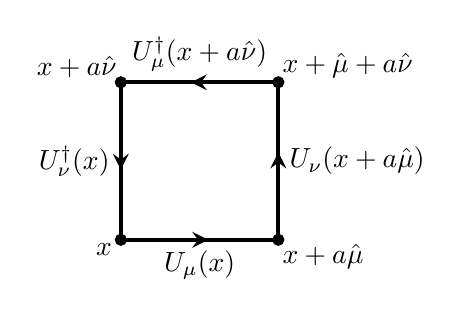
\begin{tikzpicture}
        % Coordinate dei vertici della plaquette
        \coordinate (A) at (0, 0);
        \coordinate (B) at (2, 0);
        \coordinate (C) at (2, 2);
        \coordinate (D) at (0, 2);

        \draw[-, line width=1.5pt] (A) -- (B) node[midway, below] {$U_\mu(x)$}; 
        \draw[-, line width=1.5pt] (B) -- (C) node[midway, right] {$U_\nu(x + a\hat{\mu})$};
        \draw[-, line width=1.5pt] (C) -- (D) node[midway, above] {$U^\dagger_\mu(x + a\hat{\nu})$}; 
        \draw[-, line width=1.5pt] (D) -- (A) node[midway, left]  {$U^\dagger_\nu(x)$};
    
        \draw[->, line width=1.5pt, >=stealth] (1.1, 0) -- ++(0.01, 0);  
        \draw[->, line width=1.5pt, >=stealth] (2, 1.1) -- ++(0, 0.01);
        \draw[->, line width=1.5pt, >=stealth] (0.9, 2) -- ++(-0.01, 0);
        \draw[->, line width=1.5pt, >=stealth] (0, 0.9) -- ++(0, -0.01);
    
        \filldraw (A) circle (2pt) node[below left=-2pt] {$x\,$};
        \filldraw (B) circle (2pt) node[below right=-2pt] {$x + a\hat{\mu}$};
        \filldraw (C) circle (2pt) node[above right=-2pt] {$x + \hat{\mu} + a\hat{\nu}$};
        \filldraw (D) circle (2pt) node[above left=-2pt] {$x + a\hat{\nu}$};
    \end{tikzpicture}
    \vspace{1mm}
\end{minipage}
\hspace{-6mm}
\begin{minipage}{0.6\textwidth}
    \begin{equation}\label{eq: plaquette}
        U_p(x) = 
        U_{\mu}(x) U_{\nu}(x + a\hat{\mu}) 
        U^\dagger_{\mu}(x + a\hat{\nu}) 
        U^\dagger_{\nu}(x) \, ,
    \end{equation}
\end{minipage}
and $\beta=\frac{2N_c}{g^2}$ is the lattice bare gauge coupling. Periodic Boundary Conditions (PBC) are imposed along all directions:
\begin{equation}\label{eq: PBC link}
    \begin{cases}
        \begin{aligned}
            U_\mu(\tau, \vb*{x}) &= U_\mu(\tau + N_T, \vb*{x}) \\
            U_\mu(\tau, \vb*{x}) &= U_\mu(\tau, \vb*{x} + N_s)
        \end{aligned} \, ,
    \end{cases}  \quad \forall \, \vb*{x}, \tau \, ,
\end{equation}
where $\tau$ corresponds to a single time-slice and $\vb*{x}$ is the 3D space coordinate.

The transfer matrix formalism allows to link the path-integral representation of the theory to an Hamiltonian formalism. To this end, it is useful to rewrite the Wilson action in Eq. \eqref{eq: Wilson_S} as a sum over time-slices, where the contributions coming from time-like and space-like plaquettes are separated \cite{Montvay:1994cy}
\begin{equation}
    S_g[U] = \sum_\tau L[U_i(\tau+1), U_0(\tau), U_i(\tau)] \, ,
\end{equation}
where $U_i(\tau)$ stands for the spatial links completely contained in time-slice $\tau$ and $U_0(\tau)$ corresponds to the temporal link connecting time-slices $\tau$ and $\tau+1$. The functional $L$ is defined as
\begin{equation}
    \begin{aligned}
        L[U_i(\tau+1), U_0(\tau), U_i(\tau)] &= \frac{1}{2} L_1[U_i(\tau+1)] + \frac{1}{2} L_1[U_i(\tau)] + \\
        &\qquad +L_2[U_i(\tau+1), U_0(\tau), U_i(\tau)] \, , 
    \end{aligned}
\end{equation}
where
\begin{align}
    L_1[U_i(\tau+1)] &= -\frac{\beta}{N_c} \sum_{p(\tau)} \Re \Tr U_p \, , \\
    L_2[U_i(\tau+1), U_0(\tau), U_i(\tau)] &= -\frac{\beta}{N_c} \sum_{p(\tau, \tau+1)} \Re \Tr U_p \, ,
\end{align}
with $p(\tau)$ being the space-like plaquettes contained in the time slice $\tau$ and $p(\tau, \tau+1)$ the time-like plaquette connecting time-slices $\tau$ and $\tau+1$. 

Before introducing the transfer matrix, recall that the Hilbert space of the theory is the space of all the $L^2$-complex-valued wave functions $\psi[U]$ of the space-like links $U_i(\vb*{x}) \in SU(N_c)$. This space is embedded with the following scalar product
\begin{equation}
    \braket{\phi}{\psi} = \int [D U_i] \phi^* [U_i] \psi[U_i] \, , \qquad [D U_i] \equiv \prod_{\vb*{x}} \prod_{i=1}^3 \delta U_i(\vb*{x}) \, .
\end{equation}



\printbibliography

\end{document}
